\documentclass[10pt]{article}

\usepackage[margin=1in]{geometry}
\usepackage[T1]{fontenc}
\usepackage{amsmath,amssymb}
\usepackage{booktabs}
\usepackage{microtype}
\usepackage{graphicx}
\graphicspath{{../}} % figures live in ../experiment-code/recon/ when built from paper/
\usepackage{algorithm}
\usepackage{algpseudocode}
\usepackage{hyperref}
\newcommand{\Feas}{\mathrm{Feasible}}
\newcommand{\argmax}{\operatorname*{arg\,max}}

\title{Supplementary Material\\[2pt]
\large Narrative Agency under Evidence Constraints}
\author{}
\date{}

\begin{document}
\maketitle
\renewcommand{\thetable}{S\arabic{table}}
\renewcommand{\thefigure}{S\arabic{figure}}
\renewcommand{\thealgorithm}{S\arabic{algorithm}}

\section*{S1. Related-work positioning}

This table reproduces the related-work comparison moved from the main
manuscript. It makes explicit how the framework differs from adjacent
formulations and what additional objects it represents.

\begin{table}[htbp]
\centering\scriptsize
\caption{Positioning relative to adjacent problem formulations.}
\label{tab:supp-novelty}
\resizebox{\linewidth}{!}{%
\begin{tabular}{@{}p{2.5cm}p{2.9cm}p{3.7cm}p{4.5cm}@{}}
\toprule
Prior line & Primary object & What it naturally expresses & What this framework adds \\
\midrule
Abduction / plan recognition & Hypotheses or latent plans & Rank or infer explanations from observations & An objective-invariant replay-admissible history set, followed by agent-specific selection \\
\addlinespace[2pt]
Narrative planning & Intentional plot structure & Construct a coherent story or plan toward a goal & Preserve every evidence-compatible causal history before choosing a report \\
\addlinespace[2pt]
Strategic communication & Messages, beliefs, or equilibria & Model persuasion, signaling, or deception incentives & Separate physical feasibility from self-interested testimony and interactive corroboration \\
\addlinespace[2pt]
This work & Feasible histories plus $J_i$ & Select incompatible accounts from one shared record & Express cases where each account is individually feasible, yet changing objectives or social pressure changes only the selected account \\
\bottomrule
\end{tabular}}
\end{table}

\clearpage
\section*{S2. Interactive testimony outcome summary}

This table contains the outcome summary omitted from the main manuscript to make
room for the more directly interpretable round-by-round hearing trace. The public
record is the fixed \emph{In a Grove} ``run-06'' record. The simulator, utilities,
and feasible pool remain fixed while the interaction parameters vary. The
``distinct'' count is the number of terminal causal claims. The ``incompatible''
count is the number of claims that cannot coexist with the joint profile under the
record. The symbol $\tau^\star$ denotes the simulator's reference history.

\begin{table}[htbp]
\centering
\small
\caption{Outcome summary for interactive testimony on the fixed \emph{In a Grove}
``run-06'' record.}
\label{tab:supp-hearing-summary}
\setlength{\tabcolsep}{6pt}%
\begin{tabular}{@{}lcccc@{}}
\toprule
condition & revisions & distinct & incompatible & $\tau^\star$ retained? \\
\midrule
Independent ($\beta=0$) & $0$ & $3$ & $2$ & yes \\
Corroborative ($\beta=.5,\gamma=0$) & $2$ & $1$ & $0$ & no \\
$+\,$accountability ($\beta=.5,\gamma=.2$) & $0$ & $3$ & $2$ & yes \\
\bottomrule
\end{tabular}
\end{table}

The corroborative condition collapses the three opening accounts to one and
removes the two jointly incompatible claims. Accountability prevents those
revisions by penalizing drift from the openings and restores the three-way
profile.

\clearpage
\section*{S3. Replay-learning curves}

Figure~\ref{fig:supp-ring-curves} reproduces the Ring replay-learning curves
reported as Figure~2 in the main manuscript. Each line is the median
best-feasible utility gap over eight seeds, with shading for the interquartile range.
A gap of zero is the exact enumerated optimum.

\begin{figure}[htbp]
\centering
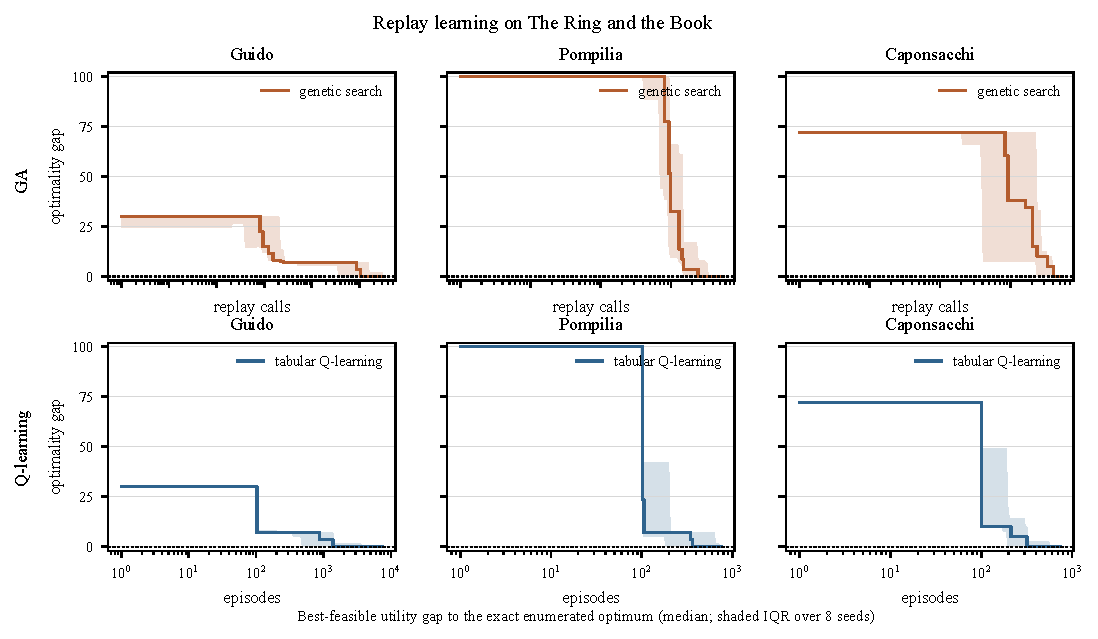
\includegraphics[width=0.96\linewidth]{experiment-code/recon/fig-ring-curves.pdf}
\caption{Empirical replay-learning curves on \emph{The Ring and the Book}.
The top row shows genetic search against replay-call budget and the bottom row
tabular Q-learning against episode budget. The curves are empirical learning
trajectories, not a formal convergence guarantee.}
\label{fig:supp-ring-curves}
\end{figure}

\clearpage
\section*{S4. Full prompting ladder and deterministic baselines}

This table gives the complete version of Table~2 from the main manuscript. The
three primary generator models use the same samples and conditions as the main
experiment. GPT-5 and Claude Opus 4.8 are separate three-sample probes. Solver
rows report their stated run or exact reference. $^{\dagger}$The account is
excluded by $F$. $^{\ddagger}$Distinct counts the three beam outputs.

\begin{table}[htbp]
\centering
\scriptsize
\caption{Full prompting ladder and deterministic baselines on \emph{In a Grove}.}
\label{tab:supp-necessity}
\resizebox{\linewidth}{!}{%
\begin{tabular}{@{}lccccc@{}}
\toprule
 & \multicolumn{3}{c}{utility attained} & & \\
\cmidrule(lr){2-4}
Solver / condition & bandit & wife & samurai & infeasible & distinct \\
\midrule
Not enforced ($\argmax$ over all assertions) & $72^{\dagger}$ & $75$ & $80$ & $23.2\%$ & $3.0$ \\
\addlinespace[1pt]
\emph{zai-glm-4.7} (instructed)                  & $48$ & $43$ & $80$ & $11.1\%$ & $3.0$ \\
\quad $+$ physical entailments spelled out       & $48$ & $43$ & $80$ & $0\%$    & $3.0$ \\
\quad $+$ self-check                             & $48$ & $43$ & $80$ & $0\%$    & $3.0$ \\
\quad $+$ self-revise                            & $48$ & $43$ & $80$ & $0\%$    & $3.0$ \\
\addlinespace[1pt]
\emph{gemma-4-31b} (instructed)                  & $48$ & $43$ & $80$ & $0\%$    & $3.0$ \\
\quad $+$ physical entailments spelled out       & $48$ & $43$ & $80$ & $0\%$    & $3.0$ \\
\quad $+$ self-check                             & $48$ & $43$ & $80$ & $11.1\%$ & $3.0$ \\
\quad $+$ self-revise                            & $48$ & $43$ & $80$ & $11.1\%$ & $3.0$ \\
\addlinespace[1pt]
\emph{gpt-oss-120b} (instructed)                 & $48$ & $75$ & $42$ & $0\%$    & $1.0$ \\
\quad $+$ physical entailments spelled out       & $48$ & $75$ & $42$ & $0\%$    & $1.0$ \\
\quad $+$ self-check                             & $48$ & $43$ & $80$ & $0\%$    & $3.0$ \\
\quad $+$ self-revise                            & $48$ & $75$ & $42$ & $0\%$    & $1.0$ \\
\addlinespace[1pt]
\emph{gpt-5} (instructed)                        & $42$ & $43$ & $80$ & $0\%$    & $3.0$ \\
\quad $+$ consequence                             & $42$ & $43$ & $80$ & $0\%$    & $3.0$ \\
\quad $+$ self-check                              & $42$ & $43$ & $80$ & $0\%$    & $3.0$ \\
\quad $+$ self-revise                             & $42$ & $43$ & $80$ & $0\%$    & $3.0$ \\
\addlinespace[1pt]
\emph{Claude Opus 4.8} (instructed)              & $42$ & $43$ & $80$ & $0\%$    & $3.0$ \\
\quad $+$ consequence                             & $42$ & $43$ & $80$ & $0\%$    & $3.0$ \\
\quad $+$ self-check                              & $42$ & $43$ & $80$ & $0\%$    & $3.0$ \\
\quad $+$ self-revise                             & $42$ & $43$ & $80$ & $11\%$   & $3.0$ \\
\addlinespace[1pt]
Constrained beam planner ($w=32$, $T=7$)         & $58$ & $75$ & $73$ & $0\%$ & $1.0^{\ddagger}$ \\
Genetic search (8 seeds)                          & $58$ & $75$ & $80$ & $0\%$ & $3.0$ \\
Tabular Q-learning (8 seeds)                     & $58$ & $75$ & $80$ & $0\%$ & $3.0$ \\
Simulator ($\argmax$ over enumerated $\Feas(F)$) & $58$ & $75$ & $80$ & $0\%$ & $3.0$ \\
\bottomrule
\end{tabular}}
\end{table}

\clearpage
\section*{S5. Utility definitions, solver protocol, and hyperparameters}

\subsection*{S5.1. Concrete definition of $U_i$}

The utility is computed entirely from the replayed causal signature, before any
language realization. For the Grove domain, replay returns six normalized
features: agency, honour, clean hands, sympathy, dignity, and wronged. Their
deterministic values are computed from the fatal actor, action type, weapon,
victim status, and whether the victim was bound or armed. The implementation
is frozen in \texttt{experiment-code/recon/grove-objective.mjs}.

The witness-specific feature triples are
\[
\begin{aligned}
U_{\mathrm{Tajomaru}}&=\tfrac{100}{3}(\mathrm{honour}+\mathrm{agency}+\mathrm{cleanHands}),\\
U_{\mathrm{Masago}}&=\tfrac{100}{3}(\mathrm{sympathy}+\mathrm{dignity}+\mathrm{cleanHands}),\\
U_{\mathrm{Takehiro}}&=\tfrac{100}{3}(\mathrm{honour}+\mathrm{agency}+\mathrm{wronged}).
\end{aligned}
\]
Each component lies in $[0,1]$, so $U_i\in[0,100]$. In particular, agency is
$1$ when the witness deals the fatal blow and $0.15$ otherwise. The clean hands
score is $0.15$ for the fatal striker and $1$ otherwise. Dignity is
$0.4+0.4\,\mathrm{agency}$. Honour is $1$ for Takehiro's self-strike, $0.6$
for an impalement on a held weapon, $0.05$ when Takehiro is bound at death,
$0.5$ when he is armed, and $0.3$ otherwise. For any other witness, honour is
$1$ when that witness makes an armed longsword strike, $0.1$ when striking a
bound victim, $0.3$ for another strike, and $0.6$ when not the fatal actor.
Sympathy is $0.35$ for the fatal striker, $0.7$ for Takehiro when not the
striker, and $0.8$ otherwise. Wronged is $0.8$ for Takehiro when another
witness strikes, $0.4$ for his self-strike, $0.6$ for his other outcomes, and
$0.3$ for the other witnesses. These rules contain no literary labels. Those
descriptions are consequences of the selected causal signature.

For the agent-operations domain, replay computes six features from the actor,
decision owner, plan author, authorization channel, intent, and monitor flag:
clean hands, non-decision, authorization, deviation, vigilance, and
vindication. The fixed triples are
Executor (authorization, non-decision, clean hands), Planner (deviation,
clean hands, non-decision), and Monitor (vigilance, vindication, clean hands).
For \emph{The Ring and the Book}, the six features are warrant, provocation,
bearing, innocence, purity, and efficacy. The fixed triples are Guido (warrant,
provocation, bearing), Pompilia (innocence, provocation, purity), and
Caponsacchi (purity, efficacy, innocence). The branch values are
deterministic functions of replayed causal fields and are listed in
\texttt{ops-objective.mjs} and \texttt{ring-objective.mjs}. No learned
parameters or language-model scores enter any $U_i$.

All non-enumerative solvers interact with a domain only through legal-action
generation, replay, evidence-miss counts, and utility evaluation. The reported
seeds are $\{1,\ldots,8\}$, using the deterministic seeded generator in the
released code. A run stops early when it reaches the exact enumerated utility.
Otherwise, it stops at the stated budget.

\begin{algorithm}[htbp]
\caption{Replay-based best-response solvers for $\hat\tau_i$ under $J_i$}
\label{alg:supp-replay}
\scriptsize
\begin{minipage}[t]{0.49\linewidth}
\textbf{(a) Genetic search}
\begin{algorithmic}[1]
\Require simulator, $F$, fixed profile $\rho_{-i}$, opening account $\tau_i^0$, objective $J_i$
\State $P \gets$ random legal histories, $A \gets \emptyset$
\For{each generation}
  \ForAll{$\tau_i \in P$}
    \State $m \gets \mathrm{misses}(\mathrm{replay}(\tau_i),F)$
    \State score $\tau_i$ by $(m,-J_i(\tau_i,\rho_{-i},\tau_i^0),|\tau_i|)$
    \State add $\tau_i$ to $A$ if $m=0$
  \EndFor
  \State $P \gets$ select/recombine/mutate/repair
  \State locally perturb the incumbent
\EndFor
\State \Return $\argmax_{\tau_i\in A} J_i(\tau_i,\rho_{-i},\tau_i^0)$
\end{algorithmic}
\end{minipage}\hfill
\begin{minipage}[t]{0.49\linewidth}
\textbf{(b) Tabular Q-learning}
\begin{algorithmic}[1]
\Require simulator, $F$, fixed profile $\rho_{-i}$, opening account $\tau_i^0$, objective $J_i$, horizon $T$
\State $Q \gets 0$, $A \gets \emptyset$
\For{each episode}
  \State reset simulator, $\tau_i \gets$ empty history
  \For{$t=1$ to $T$}
    \State choose legal $a$ by $\epsilon$-greedy $Q$
    \State append $a$ to $\tau_i$ and step simulator
  \EndFor
  \State $m \gets \mathrm{misses}(\mathrm{replay}(\tau_i),F)$
  \State $r \gets J_i(\tau_i,\rho_{-i},\tau_i^0)$ if $m=0$, else $-\lambda m$
  \State update $Q$ backward along $\tau_i$
  \State add $\tau_i$ to $A$ if $m=0$
\EndFor
\State \Return $\argmax_{\tau_i\in A} J_i(\tau_i,\rho_{-i},\tau_i^0)$
\end{algorithmic}
\end{minipage}
\end{algorithm}

\begin{table}[htbp]
\centering\scriptsize
\caption{Replay-solver hyperparameters used for the reported recovery results.}
\label{tab:supp-solver-protocol}
\resizebox{\linewidth}{!}{%
\begin{tabular}{@{}llllp{4.2cm}@{}}
\toprule
solver & domain(s) & horizon & budget & stochastic settings and stopping rule \\
\midrule
genetic search & Grove, Ops & $T=7$ & $\mathrm{POP}=40$, $\mathrm{GENS}=40$ & crossover probability $0.7$, mutation probability $0.3$, tournament size $3$, elitism, and $8$ local perturbations per generation. Stop at exact optimum or generation cap \\
genetic search & Ring & $T=24$ & $\mathrm{POP}=80$, $\mathrm{GENS}=300$ & same crossover, mutation, tournament, elitism, and local-search settings. Stop at exact optimum or generation cap \\
tabular Q-learning & Grove, Ops & $T=7$ & $6{,}000$ episodes & learning rate $\eta=0.4$, discount $\gamma_Q=0.95$, legal-action masking, and linear $\epsilon$ schedule $0.90\!\to\!0.05$. Stop at exact optimum or episode cap \\
tabular Q-learning & Ring & $T=24$ & $12{,}000$ episodes & same $\eta$, $\gamma_Q$, action masking, and $\epsilon$ schedule. Stop at exact optimum or episode cap \\
constrained beam & Grove & $T=7$ & width $w=32$ & deterministic decoding with illegal actions masked. No stochastic seed sweep \\
\bottomrule
\end{tabular}}
\end{table}

For genetic search, the primary fitness key is the number of evidence misses,
followed by utility and then shorter history length. Crossover is legalised by
replay and mutation extends a legal prefix. For Q-learning, a feasible episode
receives $1+\bar U_i$ and an infeasible episode receives $-0.2m$, where $m$ is
the number of evidence misses. The cost columns in the main solver table are
not the same unit: enumeration counts explored states, genetic search counts
simulator calls to first reach the optimum, and Q-learning counts episodes to
first reach it.

\clearpage
\section*{S6. Ring filtration and sensitivity audit}

The Ring candidate space contains $576$ distinct causal assertions before the
public record is applied. Replaying the fixed eleven-document record leaves
$36$ feasible assertions, a $93.75\%$ reduction. These are assertion counts.
The corresponding enumeration explored $32{,}928$ reachable states. The
Ring domain is derived from Browning's account of the Franceschini prosecution.
The primary-source citation appears in the main manuscript.

\begin{table}[htbp]
\centering\small
\caption{Ring assertion-space filtration under the fixed public record.}
\label{tab:supp-ring-filtration}
\begin{tabular}{@{}lrrr@{}}
\toprule
candidate assertions & feasible assertions & removed & reduction \\
\midrule
$576$ & $36$ & $540$ & $93.75\%$ \\
\bottomrule
\end{tabular}
\end{table}

For the Grove sensitivity audit, the $19$ hand-set feature constants are on a
$[0,1]$ scale. In each of $5{,}000$ trials (seed $16980222$), every constant
receives an independent offset drawn uniformly from $[-0.4,0.4]$ and is then
clipped to $[0,1]$. The simulator and feasible set remain fixed. For each trial
we recompute each witness's utility argmax over that feasible set. A trial
counts as preserving the full spread when the three selected causal signatures
are distinct. This occurs in $4{,}040/5{,}000=80.8\%$ of trials, with a $95\%$
Wilson interval of $[79.7,81.9]\%$. Thus ``$\pm0.4$'' is an absolute offset on
the normalized feature scale, not a relative percentage change.

\end{document}
